\section{Semiconduttori}
\subsection{Classificazione dei materiali}
Ressitività $\rho$:
\begin{itemize}
    \item $\rho < 10^{-1}\Omega\cdot cm$ è un conduttore
    \item $10^{-1}\Omega\cdot cm < \rho < 10^{5}\Omega\cdot cm $ è un semiconduttore
    \item $10^{5}\Omega\cdot cm < \rho$ è un isolante
\end{itemize}

\subsubsection{Caratteristiche dei semiconduttori}
\begin{itemize}
    \item resistività intermedia tra isolanti e conduttori
    \item possibilità di variare $\rho$ mediante il drogaggio
    \item due portatori di carica liberi: elettrone(-) e lacuna(+)
    \item disponibili sia come cristalli che come composti
\end{itemize}

\subsubsection{Silicio: legame covalente}
4 elettroni poco legati(di valenza)
\begin{itemize}
    \item non sono legati strettamente al nucleo
    \item risentono dell'interazione deglie altri atomi
    \item formano un doppio legame covalente con gli altri atomi
\end{itemize}

\subsection{Drogaggio di un semiconduttore}

Il drogaggio è l'aggiunta di atomi diversi, esistono 2 tipi di drogaggio:
\begin{itemize}
    \item drogaggio di tipo n: aggiunta di elementi del quinto gruppo(As,P,Sb)
    \item drogaggio di tipo p: aggiunta di elementi del terzo gruppo(B)
\end{itemize}


\subsubsection{Silicio di tipo n}
Vengono aggiunti al silicio elementi del quinto gruppo, il quinto elettrone di valenza si lega debolmente al nucle
e non è impiegato in legami covalenti.
L'elettrone può facilmente liberarisi dal nucleo per effetto dell'energia termica.


Il quinto elettrone può muoversi nel cristallo.

\subsubsection{Silicio di tipo p}
Essendo il drogaggio effettuato con un elemento del terzo gruppo, manca un elettrone nel legame
covalente(\textbf{lacuna}).

È facile catturare un elettrone per questa configurazione.

La cattura di un elettrone da parte di questa configurazione, crea una lacuna in una molecola vicina,
viene creata una rezione a catena dove questa lacuna si "sposta" all'interno degli atomi adiacenti.

Si parla di "moto di lacune" anche se sono comunque gli elettroni a muoversi.

\subsection{Corrente di "drift"}
\begin{figure}[H]
    \centering
    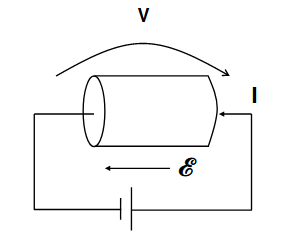
\includegraphics[width=0.3\linewidth]{imgs/corrente-di-drift}
    \caption{Corrente di drift}
    \label{fig:corrente_drift}
\end{figure}
Forza di trascinamento sull'elettrone
\begin{equation*}
    F = -q \epsilon
\end{equation*}

Forza di trascinamento sulla lacuna
\begin{equation*}
    F = q \epsilon
\end{equation*}

Per campi elettrici moderati esiste una relazione lineare fra intensità del campo
$\epsilon$ e \textbf{velocità del portatore di carica}.

Materiali ad alta mobilità($\mu$) hanno una velocità media dei portatori molto alta.


\begin{figure}[H]
    \centering
    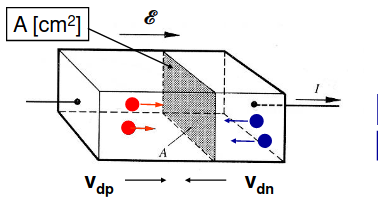
\includegraphics[width=0.3\linewidth]{imgs/corrente}
    \caption{Corrente}
    \label{fig:corrente}
\end{figure}

Dove le forse sono:
\begin{itemize}
    \item
        \begin{equation*}
            I_n = -qn(-V_{dn})A = qnV_{dn}A
        \end{equation*}
    \item
        \begin{equation*}
            I_p = qpV_{dp}A
        \end{equation*}
\end{itemize}

La $A$ sta per la superficie attraversata perchè la corrente è il numero di lacune che attraversano la superficie in un 
tempo.

La densità si ottiene dividendo per l'Area.

La J rappresenta la densità di corrente:
\begin{equation*}
    J = J_p + J_n = q(p_\mu_p + n\mu_n)\cdot \epsilon
\end{equation*}
Da cui si ottiene la legge di \textbf{ohm locale}:
\begin{equation*}
    J = \sigma \cdot \epsilon
\end{equation*}

Dove la $\sigma$ rappresenta la conducibilità:
\begin{equation}
    \sigma = \frac{1}{\rho} = q(p_\mu_p + n\mu_n)
\end{equation}
dove $\rho$ rappresenta la resistività.

\subsubsection{Drift: metalli vs semiconduttori}
Nei metalli e nei semiconduttori, il drift è simile, tranne per il fatto che nei metalli non vi sono lacune come
portatori di carica.
E ovviamente che la conducibilità di un metallo è molto maggiroe di quella di un semiconduttore.

\subsection{Diffusione}
Meccanismo di trasporto rilevante solo nei semiconduttori, simile alal diffusione dei gas causata da una
differenza di concetrazione dei portatori.

\subsubsection{Diffusione: elettroni}
 \begin{equation}
     J_n=-(-q)D_n\frac{dn}{dx} = qD_n\frac{dn}{dx}
 \end{equation}
essendo l'elettrone negativo si prende la crica q con carica negativa, il segno meno iniziale rappresenta
il flusso verso la zona a minor intensità.

\subsubsection{Diffizione: lacune}
\begin{equation}
    J_p=-qD_p\frac{dp}{dx}
\end{equation}


\subsection{Legge del trasporto "drift-diffusione"}

I due meccanismi di trasporto per le due cariche sono:
elettrone:
\begin{equation}
    J_n= qn\mu_n\epsilon + qD_n\frac{dn}{dx}
\end{equation}
lacuna:
\begin{equation}
    J_p= qp\mu_p\epsilon - qD_p\frac{dp}{dx}
\end{equation}

Il \textbf{DRIFT} tipicamente è dominante per i \textbf{maggioritari}: $J_{n-drift} \propto n\epsilon$.


La \textbf{DIFFUSIONE} tipicamente è dominante per i \textbf{minoritari}: $J_{n-diff} \propto \frac{dn}{dx}$.

